\documentclass[12pt,a4paper]{article}

\usepackage[utf8]{inputenc}
\usepackage[T1]{fontenc}

\usepackage[top=2.5cm,bottom=2.5cm,left=2.8cm,right=2.8cm]{geometry}
\usepackage[dvipsnames,svgnames,x11names]{xcolor}

\definecolor{androidgreen}{HTML}{3DDC84}
\definecolor{darkbg}{HTML}{1A0A2E}
\definecolor{lightgray}{HTML}{F5F5F5}
\definecolor{codebg}{HTML}{F0F8F4}
\definecolor{commentgreen}{HTML}{2E7D32}
\definecolor{keywordblue}{HTML}{1565C0}
\definecolor{stringorange}{HTML}{E65100}
\definecolor{linenumgray}{HTML}{9E9E9E}
\definecolor{infobg}{HTML}{E8F5E9}
\definecolor{warnbg}{HTML}{FFF8E1}
\definecolor{warnframe}{HTML}{F9A825}

\usepackage{graphicx}
\usepackage{tikz}
\usetikzlibrary{shapes.geometric,arrows.meta,positioning,calc,fit,backgrounds}
\usepackage{tcolorbox}
\tcbuselibrary{skins,breakable}

\usepackage{listings}
\lstdefinestyle{javaStyle}{
  backgroundcolor=\color{codebg},
  commentstyle=\color{commentgreen}\itshape,
  keywordstyle=\color{keywordblue}\bfseries,
  stringstyle=\color{stringorange},
  numberstyle=\tiny\color{linenumgray},
  basicstyle=\ttfamily\footnotesize,
  breaklines=true,
  keepspaces=true,
  numbers=left,
  numbersep=8pt,
  showstringspaces=false,
  tabsize=2,
  frame=none,
  xleftmargin=18pt,
  aboveskip=0pt,
  belowskip=0pt,
}
\lstset{style=javaStyle}

\usepackage{booktabs}
\usepackage{tabularx}
\usepackage{colortbl}
\usepackage{float}
\usepackage{titlesec}
\usepackage{parskip}
\usepackage[colorlinks=true,linkcolor=darkbg,urlcolor=androidgreen]{hyperref}
\usepackage{fancyhdr}

\pagestyle{fancy}
\fancyhf{}
\renewcommand{\headrulewidth}{0pt}
\fancyhead[L]{\small\color{gray}\texttt{Android Versions App}}
\fancyhead[R]{\small\color{gray}Parcial 2 --- Mayo 2026}
\fancyfoot[C]{\small\color{gray}\thepage}

\titleformat{\section}
  {\color{darkbg}\large\bfseries}{}
  {0em}
  {\colorbox{androidgreen}{\color{white}\makebox[0.5cm][c]{\thesection}}\quad}
  [\vspace{-0.3em}\textcolor{androidgreen}{\rule{\linewidth}{1.5pt}}]

\titleformat{\subsection}
  {\color{darkbg}\normalsize\bfseries}
  {\color{androidgreen}\thesubsection\;}{0em}{}

\titleformat{\subsubsection}
  {\color{darkbg}\small\bfseries\itshape}{}{0em}{}

\newtcolorbox{patternbox}[2][]{
  enhanced, breakable,
  colback=infobg, colframe=androidgreen,
  fonttitle=\bfseries\small, title=#2,
  arc=4pt, boxrule=1.5pt,
  left=8pt, right=8pt, top=6pt, bottom=6pt, #1
}

\newtcolorbox{warnbox}[1]{
  enhanced, colback=warnbg, colframe=warnframe,
  fonttitle=\bfseries\small, title=#1,
  arc=4pt, boxrule=1.5pt,
  left=8pt, right=8pt, top=6pt, bottom=6pt,
}

\newtcolorbox{infobox}{
  enhanced, colback=infobg, colframe=androidgreen,
  arc=4pt, boxrule=1pt,
  left=10pt, right=10pt, top=6pt, bottom=6pt,
}

\newtcolorbox{filebox}[1]{
  enhanced, breakable,
  colback=codebg, colframe=androidgreen!50,
  title={\texttt{#1}},
  fonttitle=\small\bfseries\ttfamily,
  coltitle=white,
  attach boxed title to top left={yshift=-2mm,xshift=6mm},
  boxed title style={colback=darkbg,arc=2pt},
  arc=4pt, boxrule=1pt,
  left=0pt, right=0pt, top=8pt, bottom=4pt,
}

%=============================================================
\begin{document}
%=============================================================

% ── Portada ──────────────────────────────────────────────────
\begin{titlepage}
\pagecolor{darkbg}
\color{white}
\centering
\vspace*{2.5cm}


\begin{tikzpicture}
  \fill[androidgreen!20,rounded corners=10pt] (-2.2,-1.8) rectangle (2.2,2.2);
  \fill[androidgreen] (-1.2,0) rectangle (1.2,1.5);
  \fill[androidgreen] (-1.8,0.2) rectangle (-1.2,1.1);
  \fill[androidgreen] (1.2,0.2) rectangle (1.8,1.1);
  \fill[androidgreen] (-0.75,-1.4) rectangle (-0.15,0);
  \fill[androidgreen] (0.15,-1.4) rectangle (0.75,0);
  \fill[androidgreen] (-1.2,1.5) .. controls (-1.2,2.1) and (1.2,2.1) .. (1.2,1.5) -- cycle;
  \fill[white] (-0.5,1.85) circle (0.17);
  \fill[white] (0.5,1.85) circle (0.17);
  \draw[androidgreen,line width=2.5pt] (-0.9,2.4) -- (-0.5,1.6);
  \draw[androidgreen,line width=2.5pt] (0.9,2.4) -- (0.5,1.6);
\end{tikzpicture}

\vspace{1.5cm}
{\fontsize{30}{36}\selectfont\bfseries Android Versions App}\\[0.5em]
{\large\color{androidgreen} Documentacion Tecnica --- Parcial 2}\\[2em]

\begin{tcolorbox}[
  enhanced, colback=white!8, colframe=androidgreen,
  arc=6pt, boxrule=1pt, width=10cm,
  left=14pt, right=14pt, top=10pt, bottom=10pt,
  center
]
\centering\color{black}
\textbf{Autor:} Diego Alejandro Groot Cabrera\\[0.4em]
\textbf{Profesor:} Adolfo Centeno \\[0.4em]
\textbf{Entrega:} 8 de Mayo de 2026
\end{tcolorbox}

\vspace{2cm}
{\color{gray}\ttfamily\small
Flutter \quad|\quad Spring Boot \quad|\quad PostgreSQL \quad|\quad Docker \quad|\quad Render}

\vfill
{\color{androidgreen!50}\rule{8cm}{0.5pt}}\\[0.5em]
{\footnotesize\color{gray} Principios de Diseno}
\end{titlepage}

\pagecolor{white}\color{black}
\newpage
\tableofcontents
\newpage

%=============================================================
\section{Descripcion General del Proyecto}
%=============================================================

\begin{infobox}
\textbf{Resumen:} Aplicacion multiplataforma para registrar versiones del
sistema operativo Android, con soporte de reacciones emoji y comentarios
por publicacion. Backend REST con Spring Boot y frontend Flutter compilado
para web, Linux desktop y APK Android.
\end{infobox}

\vspace{0.5em}

La idea del proyecto es tener una especie de red social enfocada en
versiones de Android. Cada usuario puede crear una publicacion con el
nombre de la version, su fecha, descripcion y caracteristicas. Otros
usuarios pueden reaccionar con emojis (\texttt{like, love, haha, wow, sad}) y
tambien dejar comentarios de texto.

El backend se hizo con \textbf{Spring Boot} y expone una API REST. La
base de datos es \textbf{PostgreSQL} en produccion (Aiven). El frontend
se construyo con \textbf{Flutter}, compilando la misma base de codigo para
web y APK de Android. El proyecto esta desplegado en \textbf{Render}
usando \textbf{Docker}.

%=============================================================
\section{Tecnologias Utilizadas}
%=============================================================

\begin{table}[H]
\centering
\renewcommand{\arraystretch}{1.4}
\begin{tabularx}{\textwidth}{>{\bfseries}l X}
\rowcolor{darkbg}
\multicolumn{1}{>{\color{white}\bfseries}l}{Tecnologia} &
\multicolumn{1}{>{\color{white}\bfseries}X}{Uso en el proyecto} \\
\rowcolor{lightgray}
Flutter (Dart) & Interfaz: web, Linux desktop y APK Android \\
\rowcolor{white}
Spring Boot 4 & Framework backend, expone la API REST \\
\rowcolor{lightgray}
PostgreSQL 16 & Base de datos relacional en produccion y local \\
\rowcolor{white}
Hibernate / JPA & Mapeo objeto-relacional de las entidades \\
\rowcolor{lightgray}
Docker & Contenedorizacion del backend para despliegue \\
\rowcolor{white}
Render & Plataforma de despliegue en la nube \\
\rowcolor{lightgray}
Maven & Gestion de dependencias y build del proyecto Java \\
\rowcolor{white}
GitHub & Control de versiones \\
\end{tabularx}
\caption{Stack tecnologico del proyecto}
\end{table}

%=============================================================
\section{Patrones de Diseno Utilizados}
%=============================================================

En el proyecto se utilizaron tres patrones de diseno de software:
\textbf{Facade} (estructural), \textbf{Repository} (arquitectural) y
\textbf{MVC} (arquitectural). El patron mas importante desde la perspectiva
de diseno estructural es Facade, que se analiza en profundidad en la
siguiente seccion.

%=============================================================
\section{Patron Estructural: Facade}
%=============================================================

\begin{patternbox}{?`Que es un patron estructural?}
Los \textbf{patrones estructurales} se ocupan de como se componen las
clases y los objetos para formar estructuras mas grandes. No se enfocan
en crear objetos (eso es trabajo de los patrones creacionales) ni en
como interactuan en tiempo de ejecucion (eso es trabajo de los
comportamentales). Su objetivo es simplificar las relaciones entre clases,
reducir el acoplamiento y hacer que el sistema sea mas facil de entender
y mantener. Ejemplos de patrones estructurales del catalogo GoF:
\textbf{Adapter, Bridge, Composite, Decorator, Facade, Flyweight, Proxy}.
\end{patternbox}

\vspace{0.5em}

\subsection{Definicion del patron Facade}

\begin{patternbox}{?`Que es el patron Facade?}
\textbf{Facade} (Fachada) proporciona una interfaz simplificada a un
conjunto de interfaces en un subsistema. Define una interfaz de nivel
superior que hace que el subsistema sea mas facil de usar. En lugar de
que el cliente tenga que conocer y coordinar multiples clases internas,
habla con una sola clase fachada que lo resuelve todo internamente.
\end{patternbox}

La analogia clasica es la de un cajero automatico: el usuario solo
presiona botones, sin saber que por detras hay comunicacion con el
banco, verificacion de saldo, actualizacion de registros contables y
emision de comprobantes. Toda esa complejidad esta \textit{detras de la fachada}.

\subsection{Estructura general del patron}

\begin{center}
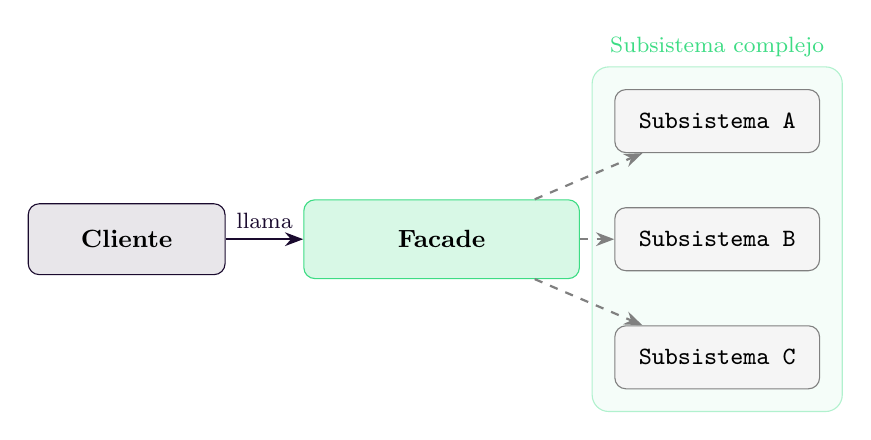
\begin{tikzpicture}[
  client/.style={draw=darkbg,fill=darkbg!10,rounded corners=4pt,
                 minimum width=2.5cm,minimum height=0.9cm,
                 font=\small\bfseries,align=center},
  facade/.style={draw=androidgreen,fill=androidgreen!20,rounded corners=4pt,
                 minimum width=3.5cm,minimum height=1cm,
                 font=\small\bfseries,align=center},
  subsys/.style={draw=gray,fill=lightgray,rounded corners=4pt,
                 minimum width=2.6cm,minimum height=0.8cm,
                 font=\small\ttfamily,align=center},
  arrow/.style={-Stealth,thick},
  darrow/.style={-Stealth,thick,color=gray,dashed}
]
\node[client] (client) at (-4,0) {Cliente};
\node[facade] (facade) at (0,0) {Facade};
\node[subsys] (s1) at (3.5, 1.5)  {Subsistema A};
\node[subsys] (s2) at (3.5, 0)    {Subsistema B};
\node[subsys] (s3) at (3.5,-1.5)  {Subsistema C};

\draw[arrow,color=darkbg] (client) -- node[above,font=\footnotesize]{llama} (facade);
\draw[darrow] (facade) -- (s1);
\draw[darrow] (facade) -- (s2);
\draw[darrow] (facade) -- (s3);

\begin{pgfonlayer}{background}
  \node[draw=androidgreen!40,fill=androidgreen!5,rounded corners=6pt,
        fit=(s1)(s2)(s3),inner sep=8pt,
        label={[font=\footnotesize\color{androidgreen}]above:Subsistema complejo}] {};
\end{pgfonlayer}
\end{tikzpicture}
\end{center}

\subsection{Por que se uso en este proyecto?}

Sin un Facade, cada controlador REST tendria que importar directamente
\texttt{AndroidRepository}, \texttt{ComentarioRepository} y
\texttt{ReaccionRepository}, y ademas conocer la logica de como
buscar un tweet, validar que existe, crear la entidad relacionada y
guardarla. Eso genera \textbf{acoplamiento fuerte}: si cambia la
logica de almacenamiento, hay que modificar cada controlador.

Con \texttt{TweetFacade}, los controladores solo conocen a la fachada
y le delegan todo. La fachada \textit{esconde} la complejidad de
coordinar tres repositorios.

\subsection{Problema sin Facade vs. solucion con Facade}

\begin{warnbox}{Sin Facade: controlador acoplado a multiples repositorios}
\begin{lstlisting}[language=Java]
// SIN FACADE - el controlador tiene que conocer TODOS los repositorios
@RestController
public class ComentarioController {
    // Acoplado a 3 repositorios directamente
    private final AndroidRepository tweetRepo;
    private final ComentarioRepository comentarioRepo;
    private final ReaccionRepository reaccionRepo;

    @PostMapping("/{id}/comentarios")
    public ResponseEntity<?> agregar(@PathVariable Long id,
                                     @RequestBody Map<String,String> body) {
        // Logica duplicada en cada controlador
        android_tweet tweet = tweetRepo.findById(id)
            .orElseThrow(() -> new RuntimeException("No existe"));
        Comentario c = new Comentario(body.get("texto"), tweet);
        comentarioRepo.save(c);
        return ResponseEntity.ok(c);
    }
}
\end{lstlisting}
\end{warnbox}

\begin{patternbox}{Con Facade: controlador simple y logica centralizada}
\begin{lstlisting}[language=Java]
// CON FACADE - el controlador solo conoce a TweetFacade
@RestController
public class ComentarioController {
    private final TweetFacade tweetFacade; // UNA sola dependencia

    @PostMapping("/{id}/comentarios")
    public ResponseEntity<?> agregar(@PathVariable Long id,
                                     @RequestBody Map<String,String> body) {
        // Solo delega, no sabe como funciona internamente
        Comentario c = tweetFacade.agregarComentario(id, body.get("texto"));
        return ResponseEntity.ok(c);
    }
}
\end{lstlisting}
\end{patternbox}

\subsection{Codigo implementado: TweetFacade}

Esta es la clase fachada real del proyecto. Coordina los tres repositorios
internamente y expone metodos simples y cohesivos:

\begin{filebox}{TweetFacade.java --- La Fachada}
\begin{lstlisting}[language=Java]
@Service
public class TweetFacade {

    // Los tres subsistemas que la fachada coordina
    private final AndroidRepository tweetRepository;
    private final ComentarioRepository comentarioRepository;
    private final ReaccionRepository reaccionRepository;

    public TweetFacade(AndroidRepository tweetRepository,
                       ComentarioRepository comentarioRepository,
                       ReaccionRepository reaccionRepository) {
        this.tweetRepository = tweetRepository;
        this.comentarioRepository = comentarioRepository;
        this.reaccionRepository = reaccionRepository;
    }

    // Operacion 1: agregar comentario (busca tweet + crea + guarda)
    public Comentario agregarComentario(Long tweetId, String texto) {
        android_tweet tweet = tweetRepository.findById(tweetId)
            .orElseThrow(() -> new RuntimeException(
                "Error: El Tweet con ID " + tweetId
                + " no existe en la DB."));
        Comentario comentario = new Comentario(texto, tweet);
        return comentarioRepository.save(comentario);
    }

    // Operacion 2: listar comentarios de un tweet
    public List<Comentario> obtenerComentarios(Long tweetId) {
        return comentarioRepository.findByTweetId(tweetId);
    }

    // Operacion 3: agregar reaccion (busca tweet + crea + guarda)
    public Reaccion agregarReaccion(Long tweetId, String tipo) {
        android_tweet tweet = tweetRepository.findById(tweetId)
            .orElseThrow(() -> new RuntimeException(
                "Tweet no encontrado"));
        Reaccion reaccion = new Reaccion(tipo, tweet);
        return reaccionRepository.save(reaccion);
    }

    // Operacion 4: listar reacciones
    public List<Reaccion> obtenerReacciones(Long tweetId) {
        return reaccionRepository.findByTweetId(tweetId);
    }

    // Operacion 5: contar reacciones por tipo (like:5, love:2, ...)
    public Map<String, Long> contarReacciones(Long tweetId) {
        List<Reaccion> reacciones =
            reaccionRepository.findByTweetId(tweetId);
        Map<String, Long> conteo = new java.util.HashMap<>();
        for (Reaccion r : reacciones) {
            conteo.merge(r.getTipo(), 1L, Long::sum);
        }
        return conteo;
    }
}
\end{lstlisting}
\end{filebox}

\subsection{Codigo implementado: Controladores que usan la Facade}

\begin{filebox}{ComentarioController.java}
\begin{lstlisting}[language=Java]
@CrossOrigin(origins = "*")
@RestController
@RequestMapping("/api/tweets")
public class ComentarioController {

    private final TweetFacade tweetFacade;

    public ComentarioController(TweetFacade tweetFacade) {
        this.tweetFacade = tweetFacade;
    }

    @PostMapping("/{id}/comentarios")
    public ResponseEntity<?> agregar(
            @PathVariable Long id,
            @RequestBody Map<String, String> body) {
        try {
            Comentario c = tweetFacade.agregarComentario(
                id, body.get("texto"));
            return ResponseEntity.ok(c);
        } catch (RuntimeException e) {
            return ResponseEntity.status(404)
                .body(Map.of("error", e.getMessage()));
        }
    }

    @GetMapping("/{id}/comentarios")
    public ResponseEntity<List<Comentario>> listar(
            @PathVariable Long id) {
        return ResponseEntity.ok(
            tweetFacade.obtenerComentarios(id));
    }
}
\end{lstlisting}
\end{filebox}

\begin{filebox}{ReaccionController.java}
\begin{lstlisting}[language=Java]
@CrossOrigin(origins = "*")
@RestController
@RequestMapping("/api/tweets")
public class ReaccionController {

    private final TweetFacade tweetFacade;

    public ReaccionController(TweetFacade tweetFacade) {
        this.tweetFacade = tweetFacade;
    }

    @PostMapping("/{id}/reacciones")
    public ResponseEntity<?> reaccionar(
            @PathVariable Long id,
            @RequestBody Map<String, String> body) {
        try {
            Reaccion r = tweetFacade.agregarReaccion(
                id, body.get("tipo"));
            return ResponseEntity.ok(r);
        } catch (RuntimeException e) {
            return ResponseEntity.status(404)
                .body(Map.of("error", e.getMessage()));
        }
    }

    @GetMapping("/{id}/reacciones")
    public ResponseEntity<List<Reaccion>> listar(
            @PathVariable Long id) {
        return ResponseEntity.ok(
            tweetFacade.obtenerReacciones(id));
    }

    @GetMapping("/{id}/reacciones/conteo")
    public ResponseEntity<Map<String, Long>> conteo(
            @PathVariable Long id) {
        return ResponseEntity.ok(
            tweetFacade.contarReacciones(id));
    }
}
\end{lstlisting}
\end{filebox}

\subsection{Diagrama UML del patron Facade en el proyecto}

El siguiente diagrama muestra como \texttt{TweetFacade} actua como la
unica puerta de entrada que los controladores usan para acceder al
subsistema de repositorios y modelos:

\begin{center}
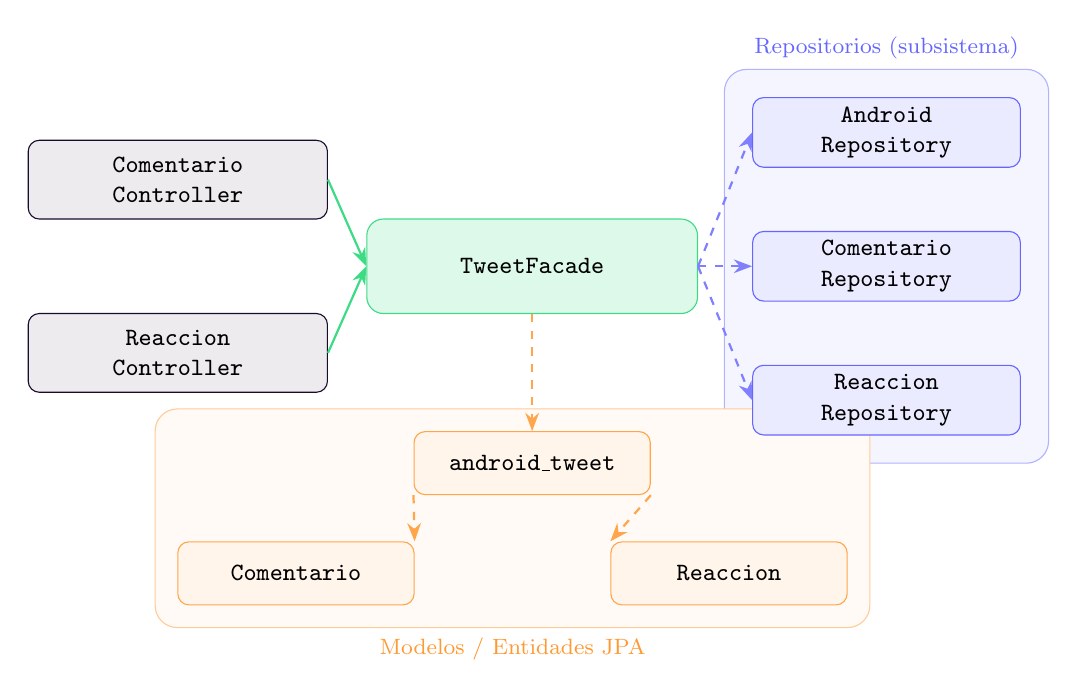
\begin{tikzpicture}[
  ctrl/.style={draw=darkbg,fill=darkbg!8,rounded corners=4pt,
               minimum width=3.8cm,minimum height=1cm,
               font=\small\ttfamily,align=center},
  facade/.style={draw=androidgreen,fill=androidgreen!18,rounded corners=6pt,
                 minimum width=4.2cm,minimum height=1.2cm,
                 font=\small\bfseries\ttfamily,align=center},
  repo/.style={draw=blue!60,fill=blue!8,rounded corners=4pt,
               minimum width=3.4cm,minimum height=0.85cm,
               font=\small\ttfamily,align=center},
  model/.style={draw=orange!70,fill=orange!8,rounded corners=4pt,
                minimum width=3.0cm,minimum height=0.8cm,
                font=\small\ttfamily,align=center},
  arrow/.style={-Stealth,thick,color=androidgreen},
  darrow/.style={-Stealth,thick,color=blue!50,dashed},
  marrow/.style={-Stealth,thick,color=orange!70,dashed}
]

% Controladores (izquierda)
\node[ctrl] (cc) at (0, 2.2)  {Comentario\\Controller};
\node[ctrl] (rc) at (0, 0)    {Reaccion\\Controller};

% Facade (centro)
\node[facade] (tf) at (4.5, 1.1) {TweetFacade};

% Repositorios (derecha arriba)
\node[repo] (ar) at (9, 2.8)  {Android\\Repository};
\node[repo] (cr) at (9, 1.1)  {Comentario\\Repository};
\node[repo] (rr) at (9,-0.6)  {Reaccion\\Repository};

% Modelos (derecha abajo)
\node[model] (at) at (4.5,-1.4) {android\_tweet};
\node[model] (cm) at (1.5,-2.8) {Comentario};
\node[model] (rm) at (7.0,-2.8) {Reaccion};

% Flechas controladores -> facade
\draw[arrow] (cc.east) -- (tf.west);
\draw[arrow] (rc.east) -- (tf.west);

% Flechas facade -> repositorios
\draw[darrow] (tf.east) -- (ar.west);
\draw[darrow] (tf.east) -- (cr.west);
\draw[darrow] (tf.east) -- (rr.west);

% Flechas facade -> modelos
\draw[marrow] (tf.south) -- (at.north);
\draw[marrow] (at.south west) -- (cm.north east);
\draw[marrow] (at.south east) -- (rm.north west);

% Etiqueta subsistema
\begin{pgfonlayer}{background}
  \node[draw=blue!30,fill=blue!4,rounded corners=8pt,
        fit=(ar)(cr)(rr),inner sep=10pt,
        label={[font=\footnotesize\color{blue!60}]above:Repositorios (subsistema)}] {};
  \node[draw=orange!40,fill=orange!4,rounded corners=8pt,
        fit=(at)(cm)(rm),inner sep=8pt,
        label={[font=\footnotesize\color{orange!80}]below:Modelos / Entidades JPA}] {};
\end{pgfonlayer}

\end{tikzpicture}
\end{center}

\subsection{Beneficios obtenidos del patron Facade}

\begin{table}[H]
\centering
\renewcommand{\arraystretch}{1.5}
\begin{tabularx}{\textwidth}{>{\bfseries}l X}
\rowcolor{darkbg}
\multicolumn{1}{>{\color{white}\bfseries}l}{Beneficio} &
\multicolumn{1}{>{\color{white}\bfseries}X}{Impacto en el proyecto} \\
\rowcolor{infobg}
Bajo acoplamiento & Los controladores no dependen de los repositorios directamente \\
\rowcolor{white}
Unico punto de cambio & Si cambia la logica de comentarios, solo se modifica \texttt{TweetFacade} \\
\rowcolor{infobg}
Codigo limpio & Cada controlador tiene menos de 30 lineas de codigo \\
\rowcolor{white}
Logica centralizada & El conteo de reacciones por tipo vive en un solo lugar \\
\rowcolor{infobg}
Facil de testear & Se puede hacer mock de \texttt{TweetFacade} sin levantar repositorios \\
\end{tabularx}
\caption{Beneficios del patron Facade en el proyecto}
\end{table}

%=============================================================
\section{Patron Repository}
%=============================================================

\begin{patternbox}{?`Que es el patron Repository?}
El Repository actua como una coleccion de objetos en memoria. En lugar
de escribir SQL directamente en la logica de negocio, se crea una
interfaz que define que operaciones se pueden hacer con cada entidad.
Spring Data JPA genera automaticamente la implementacion a partir
del nombre de los metodos, sin necesidad de escribir SQL.
\end{patternbox}

\subsubsection{Repositorios implementados}

\begin{filebox}{ComentarioRepository.java}
\begin{lstlisting}[language=Java]
@Repository
public interface ComentarioRepository
        extends JpaRepository<Comentario, Long> {

    // Spring genera automaticamente:
    // SELECT * FROM comentarios WHERE tweet_id = ?
    List<Comentario> findByTweetId(Long tweetId);
}
\end{lstlisting}
\end{filebox}

\begin{filebox}{ReaccionRepository.java}
\begin{lstlisting}[language=Java]
@Repository
public interface ReaccionRepository
        extends JpaRepository<Reaccion, Long> {

    // SELECT * FROM reacciones WHERE tweet_id = ?
    List<Reaccion> findByTweetId(Long tweetId);

    // SELECT COUNT(*) FROM reacciones WHERE tweet_id = ?
    long countByTweetId(Long tweetId);
}
\end{lstlisting}
\end{filebox}

\begin{filebox}{AndroidRepository.java}
\begin{lstlisting}[language=Java]
@Repository
public interface AndroidRepository
        extends JpaRepository<android_tweet, Long> {

    // SELECT * FROM android_versions WHERE user_id = ?
    List<android_tweet> findByUserId(Long userId);
}
\end{lstlisting}
\end{filebox}

\begin{filebox}{UserRepository.java}
\begin{lstlisting}[language=Java]
@Repository
public interface UserRepository
        extends JpaRepository<User, Long> {

    // SELECT * FROM users WHERE correo = ?
    Optional<User> findByCorreo(String correo);

    // SELECT COUNT(*) > 0 FROM users WHERE correo = ?
    boolean existsByCorreo(String correo);
}
\end{lstlisting}
\end{filebox}

%=============================================================
\section{Modelos / Entidades JPA}
%=============================================================

Los modelos son clases Java anotadas con \texttt{@Entity} que Hibernate
mapea automaticamente a tablas de PostgreSQL.

\begin{filebox}{android\_tweet.java --- Entidad principal}
\begin{lstlisting}[language=Java]
@Entity
@Table(name = "android_versions")
public class android_tweet {

    @Id
    @GeneratedValue(strategy = GenerationType.IDENTITY)
    private Long id;

    @NotBlank @Size(max = 100)
    private String nombre;

    @NotBlank
    private String fecha;

    @NotBlank @Size(max = 500)
    private String descripcion;

    @Column(length = 1000)
    private String caracteristicas;

    @Column(name = "url_photo")
    private String urlPhoto;

    // Relacion: muchas versiones pertenecen a un usuario
    @ManyToOne(fetch = FetchType.LAZY)
    @JoinColumn(name = "user_id")
    @JsonIgnore
    private User user;
}
\end{lstlisting}
\end{filebox}

\begin{filebox}{Comentario.java}
\begin{lstlisting}[language=Java]
@Entity
@Table(name = "comentarios")
public class Comentario {

    @Id
    @GeneratedValue(strategy = GenerationType.IDENTITY)
    private Long id;

    private String texto;

    // Relacion: muchos comentarios pertenecen a un tweet
    @ManyToOne(fetch = FetchType.LAZY)
    @JoinColumn(name = "tweet_id")
    @JsonIgnore  // Evita referencia circular en la serializacion JSON
    private android_tweet tweet;
}
\end{lstlisting}
\end{filebox}

\begin{filebox}{Reaccion.java}
\begin{lstlisting}[language=Java]
@Entity
@Table(name = "reacciones")
public class Reaccion {

    @Id
    @GeneratedValue(strategy = GenerationType.IDENTITY)
    private Long id;

    private String tipo; // "like", "love", "haha", "wow", "sad"

    // Relacion: muchas reacciones pertenecen a un tweet
    @ManyToOne(fetch = FetchType.LAZY)
    @JoinColumn(name = "tweet_id")
    @JsonIgnore
    private android_tweet tweet;
}
\end{lstlisting}
\end{filebox}

\begin{filebox}{User.java}
\begin{lstlisting}[language=Java]
@Entity
@Table(name = "users")
public class User {

    @Id
    @GeneratedValue(strategy = GenerationType.IDENTITY)
    private Long id;

    @NotBlank
    private String nombre;

    @NotBlank
    @Column(unique = true)
    private String correo;

    @NotBlank
    private String contrasena;

    // Un usuario puede tener muchas versiones de Android
    @OneToMany(mappedBy = "user", cascade = CascadeType.ALL)
    @JsonIgnore
    private List<android_tweet> versiones = new ArrayList<>();
}
\end{lstlisting}
\end{filebox}

%=============================================================
\section{Patron MVC}
%=============================================================

\begin{patternbox}{?`Que es el patron MVC?}
MVC divide la aplicacion en tres capas: el \textbf{Modelo} maneja
los datos, la \textbf{Vista} muestra la interfaz al usuario, y el
\textbf{Controlador} recibe las peticiones y coordina entre los otros
dos. Esto permite cambiar la interfaz sin tocar la logica del negocio.
\end{patternbox}

En este proyecto MVC se aplica en dos niveles simultaneos:

\begin{itemize}
  \item \textbf{Backend (Spring Boot):} las entidades JPA son el Modelo,
        los \texttt{@RestController} son los Controladores, y el JSON
        que retorna la API es la representacion de la Vista.
  \item \textbf{Frontend (Flutter):} los widgets de Flutter son la Vista
        que consume la API y muestra los datos al usuario.
\end{itemize}

%=============================================================
\section{Endpoints de la API REST}
%=============================================================

\begin{table}[H]
\centering
\renewcommand{\arraystretch}{1.4}
\begin{tabularx}{\textwidth}{>{\ttfamily\footnotesize}l
                              >{\ttfamily\footnotesize}l X}
\rowcolor{darkbg}
\multicolumn{1}{>{\color{white}\bfseries\rmfamily\small}l}{Metodo} &
\multicolumn{1}{>{\color{white}\bfseries\rmfamily\small}l}{Ruta} &
\multicolumn{1}{>{\color{white}\bfseries\rmfamily\small}X}{Descripcion} \\
\rowcolor{androidgreen!15}
\multicolumn{3}{l}{\textbf{\small Versiones de Android}} \\
GET    & /api/android-versions?userId=\{id\} & Obtener versiones de un usuario \\
\rowcolor{lightgray}
POST   & /api/android-versions?userId=\{id\} & Crear nueva version \\
DELETE & /api/android-versions/\{id\}        & Eliminar version por ID \\
\rowcolor{androidgreen!15}
\multicolumn{3}{l}{\textbf{\small Usuarios}} \\
\rowcolor{lightgray}
POST   & /api/users            & Registrar nuevo usuario \\
POST   & /api/users/login      & Iniciar sesion \\
PUT    & /api/users/\{id\}     & Actualizar datos del usuario \\
\rowcolor{lightgray}
DELETE & /api/users/\{id\}     & Eliminar cuenta \\
\rowcolor{androidgreen!15}
\multicolumn{3}{l}{\textbf{\small Reacciones y Comentarios (via Facade)}} \\
\rowcolor{lightgray}
POST   & /api/tweets/\{id\}/reacciones         & Agregar reaccion \\
GET    & /api/tweets/\{id\}/reacciones/conteo  & Conteo por tipo \\
\rowcolor{lightgray}
POST   & /api/tweets/\{id\}/comentarios        & Agregar comentario \\
GET    & /api/tweets/\{id\}/comentarios        & Lista de comentarios \\
\end{tabularx}
\caption{Endpoints completos de la API REST}
\end{table}

%=============================================================
\section{Arquitectura y Despliegue}
%=============================================================

\begin{center}
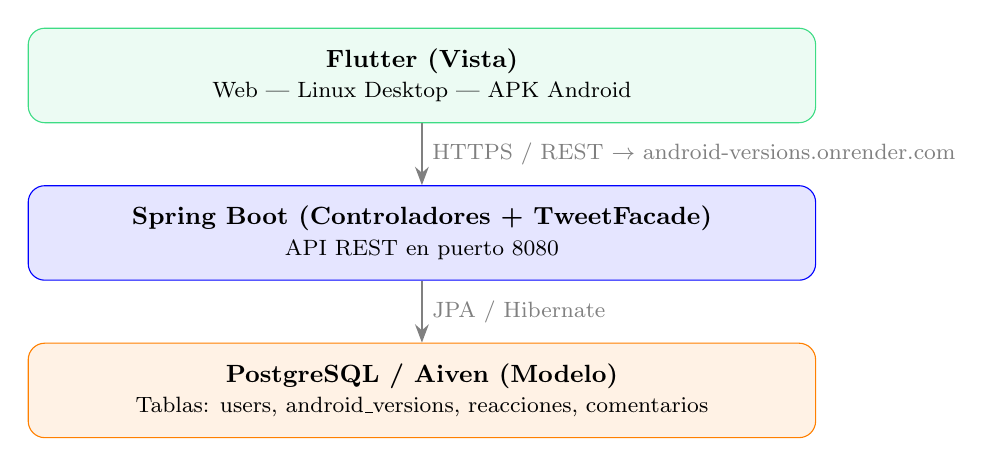
\begin{tikzpicture}[
  layer/.style={draw=#1,fill=#1!10,rounded corners=6pt,
                minimum width=10cm,minimum height=1.2cm,
                font=\small\bfseries,align=center},
  arrow/.style={-Stealth,thick,color=gray}
]
\node[layer=androidgreen] (flutter) at (0,4)
  {Flutter (Vista)\\
   \footnotesize\normalfont Web --- Linux Desktop --- APK Android};
\node[layer=blue] (spring) at (0,2)
  {Spring Boot (Controladores + TweetFacade)\\
   \footnotesize\normalfont API REST en puerto 8080};
\node[layer=orange] (db) at (0,0)
  {PostgreSQL / Aiven (Modelo)\\
   \footnotesize\normalfont Tablas: users, android\_versions, reacciones, comentarios};
\draw[arrow] (flutter) -- node[right,font=\footnotesize]{HTTPS / REST $\rightarrow$ android-versions.onrender.com} (spring);
\draw[arrow] (spring) -- node[right,font=\footnotesize]{JPA / Hibernate} (db);
\end{tikzpicture}
\end{center}

\vspace{0.5em}

El backend se empaqueta con Maven en un JAR y se contenedoriza con Docker.
Las variables de entorno \texttt{DATABASE\_URL}, \texttt{DB\_USER} y
\texttt{DB\_PASSWORD} configuran la conexion a Aiven desde Render.

\begin{tcolorbox}[
  enhanced, colback=darkbg, colframe=androidgreen,
  arc=4pt, boxrule=1pt,
  left=10pt, right=10pt, top=8pt, bottom=8pt,
]
\color{androidgreen}\ttfamily\small
\# Desarrollo local\\
\$ mvn spring-boot:run -Dspring-boot.run.profiles=local\\[4pt]
\# Produccion (Render lo ejecuta automaticamente via Docker)\\
\$ flutter build web --release \quad\# frontend web\\
\$ flutter build apk --release \quad\# APK Android
\end{tcolorbox}

%=============================================================
\section{Conclusion}
%=============================================================

El patron \textbf{Facade} fue el aporte estructural mas importante del
proyecto. Al encapsular toda la coordinacion entre \texttt{AndroidRepository},
\texttt{ComentarioRepository} y \texttt{ReaccionRepository} dentro de
\texttt{TweetFacade}, se logro que los controladores REST quedaran con
una sola dependencia y menos de 30 lineas de codigo cada uno. Eso hace
el sistema mas facil de mantener: si la logica de conteo de reacciones
cambia, solo se modifica la fachada.

Los \textbf{repositorios} eliminaron la necesidad de escribir SQL, ya que
Spring Data JPA genera las consultas automaticamente a partir del nombre
de los metodos como \texttt{findByTweetId} o \texttt{existsByCorreo}.

El patron \textbf{MVC} permitio desarrollar el backend (Spring Boot) y
el frontend (Flutter) de forma completamente independiente, comunicandose
unicamente a traves de la API REST desplegada en Render.

\end{document}